\documentclass[a4paper,12pt,draft,DIV=calc]{scrartcl}

% Character Encoding
\usepackage[utf8]{inputenc}
\usepackage[T1]{fontenc}

% Math Typesetting
\usepackage{amsmath}

% URLs
\usepackage{url}
\usepackage[pdfusetitle,hidelinks]{hyperref}

% Various Typesetting Packages
\usepackage{microtype}
\usepackage[british]{babel}

% Tikz
\usepackage{tikz}
\usetikzlibrary{positioning}

% Code references (command is mainly used so I can keep track of them easily)
\newcommand{\coderef}[3]{\emph{(#1, #2, #3)}}

\begin{document}
% Title
\title{EMBS WSN MAC Layer Protocol Report}
\author{James Cowgill}
\date{27th November 2015}
\maketitle

\section{Overview Stuff}
Report entry 1:
 - Design + Implementation Decisions
   - Synchronizing to multiple sinks
   + Handling of sinks with n = 1
 - References of the form (class name, method name, line numbers)
   - For every decision
 - Max 400 words, does not include references and figures
 + "well illustrated"

Report entry 2:
 - Design + Implementation Decisions
   - Synchronizing to multiple sinks
   - Design decisions related to energy efficiency
 - References as above
 - Max 500 words as above

\section{Exercise 1 - Ptolemy II}
\begin{figure}[ht]
  \centering
  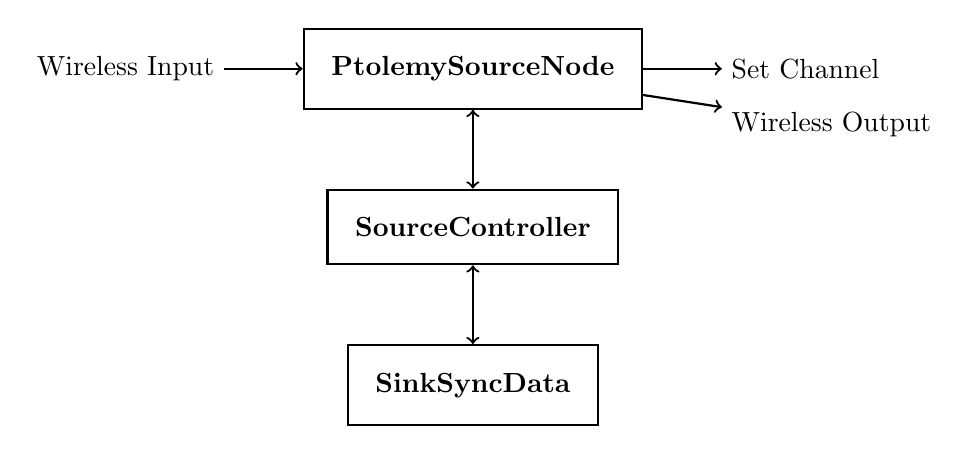
\begin{tikzpicture}[
     class/.style={draw, rectangle, thick, align=center, inner sep=1em,
		   font=\bfseries},
     port/.style={},
     arrow/.style={thick}]

    \node(SourceNode)       [class] {PtolemySourceNode};
    \node(SourceController) [class,below=of SourceNode] {SourceController}
      edge [<->,arrow] (SourceNode);
    \node(SinkSyncData)     [class,below=of SourceController] {SinkSyncData}
      edge [<->,arrow] (SourceController);

    \node(inWifi)           [port,left=of SourceNode] {Wireless Input}
      edge [->,arrow] (SourceNode);
    \node(setChannel)       [port,right=of SourceNode] {Set Channel}
      edge [<-,arrow] (SourceNode);
    \node(outWifi)          [port,below=2em of setChannel.west,anchor=west]
      {Wireless Output} edge [<-,arrow] (SourceNode);
  \end{tikzpicture}
  \caption{Exercise 1 Block Diagram}
\end{figure}

The design for the system I implemented for Exercise 1 is split into 3 classes to
try and modularize the code and separate the different tasks:
\begin{description}
  \item[SinkSyncData]
    Controls the synchronization with one specific sink, and calculates when
    the reception period is from the data it's gathered.
  \item[SourceController]
    Coordinates multiple SinkSyncData objects (one for each sink), and
    controls which channel to listen for beacons on.
  \item[PtolemySourceNode]
    Contains the Ptolemy specific code for the implementation. Most events are
    forwarded to an instance of SourceController to do any calculations.
\end{description}

\subsection{SinkSyncData}

%%%%%%%%%%%%%%%%%%%%%%% SOME INTRO HERE?

From the initial problem, it is possible to derive a function giving the exact
time each beacon frame will be received by the source.

\begin{equation*}
  f(s, n, t, i, b) = ((11 + n)i - (b - 1)t + s
\end{equation*}
\begin{description}
  \item[$s$] Absolute start time
  \item[$n$] Value of n from the protocol, number of beacons to be sent
  \item[$t$] Value of t from the protocol, time between beacons
  \item[$i$] Integer iteration number
  \item[$b$] Integer beacon number within this iteration (1 \dots $n$)
\end{description}

This function gives the absolute time a beacon occurs, but to eliminate the
value of $s$ we will subtract the times of two beacons received from a
particular sink. The function giving the time between beacons simplifies to:
\begin{align*}
  \Delta t &= f(s, n, t, i_2, b_2) - f(s, n, t, i_1, b_1) \\
           &= ((11 + n)(i_2 - i_1) - b_2 + b_1)t
\end{align*}

This is then used within the receiveBeacon function \coderef{SinkSyncData}
{receiveBeacon}{78-149} to calculate good values for $n$ and $t$. By recording
the time and $n$ value of the previous beacon, we will always know the values
of $\Delta t$, $b_1$ and $b_2$. The main part of the algorithm works roughly
like this:

\begin{enumerate}
  \item Update the best $n$ value we've received so far.
  \item If we receive two beacons which are close enough to know they are
    definitely from the same iteration, we can immediately calculate the value
		of $t$ knowing that $i_2 = i_1$ using $t = \frac{\Delta t}{b_1 - b_2}$.
	\item If the two beacons are far apart, it is more difficult to calculate the
		value of $t$ for certain (we probably don't know the final value of $n$,
		an iteration may have elapsed between the beacons). However, we can make
		some estimates which are likely to be right. These can be changed later if
		a more useful pair of beacons are received.
		\begin{enumerate}
			\item If the second beacon could be from the same iteration, guess
				using the same value of $t$ as above.
			\item If the second beacon is definitely from another iteration, and our
				current best value for $n = 1$, try calculating $t$ assuming that only
				one iteration has passed using $t = \frac{\Delta t}{11 + n + b_1 -
				b_2}$. This is the only reasonable thing to do when $n = 1$ since we
				have no other beacons from the same iteration, although it might give
				the wrong result if we "miss out" a beacon.
		\end{enumerate}
	\item If we know the value of $t$ and we have two beacons from sequential
		iterations, we can calculate the value of $n$ exactly, even if we miss a
		beacon from the second iteration. Rearranging the $\Delta t$ function gives
		$x = (11 + n)(i_2 - i_1) = \frac{\Delta	t}{t} - (b_1 - b_2)$. Knowing that
		$n \leq 10$, the easiest solution is $n = x - 11$ for $12 \leq x \leq 21$.
\end{enumerate}

% Explain how n + 1 case is handled by the above algorithm.

\subsection{SourceController}


\subsection{PtolemySourceNode}
This class contains the Ptolemy specific code. All the interesting parts of the
model are implemented in Java here (only connections to wireless ports are
outside the class).

When the actor is fired, any beacons received are forwarded to the
SourceController instance \coderef{PtolemySourceNode}{fire}{136-146} and any
packets to be sent and channel changes are handled. In Ptolemy, changing the
channel can happen at any time, but it's not possible to send two packets to
different channels within the same fire event. To workaround this, whenever a
packet is sent, the actor fires itself so it can handle any subsequent packets
\coderef{PtolemySourceNode}{sendPendingPacket}{106-112}.

Timer events are also handled by the actor firing itself, but since the time
until the actor wakes up could decrease (e.g. if we receive an $n = 1$ beacon,
we might need to transmit a packet in a short time), the time is recorded so
that any spurious timer events can be dropped.

\section{Exercise 2 - Mote Runner}
For the second exercise, I chose to reuse the back end parts of the code I wrote
for Ptolemy. This was enabled since both Ptolemy and Mote Runner can be
programmed in Java. Reusing the code meant I had to write much less code in
total, and allows simulation in Ptolemy of the actual code in the final
implementation. Since the code for Ptolemy was designed to take into account the
loss of random beacons (since SourceController can change the channel at will),
the code should still work in the real world where beacons can be lost for
various reasons during normal operation.

The implementation for exercise 2 revolves around the
handleControllerStateChange method
\coderef{MoteSourceNode}{handleControllerStateRef}{192-250}. This method is
called after each type of event has been processed to try and update the state
of the radio to what the SourceController class wants. Most actions (such as the
scheduling of a timer event, starting the receiver and transmitting packets) are
initiated here.
% ^^ WHY?

Unlike the Ptolemy model, it is not possible to change the channel of the Mote
Runner radio while receiving or transmitting. To workaround this, the state of
the radio is recorded in two variables (txOn and rxOn), and the tryChangeChannel
method \coderef{MoteSourceNode}{tryChangeChannel}{252-284} will only attempt to
change channels if these variables are false. Otherwise it will wait for the
radio to finish, and the call to tryChangeChannel will be retried later.

\end{document}
